\section{Inverted Pendulum Hardware}
The following section describes the hardware connected to the inverted pendulum setup illustrated cf. figure \ref{fig:InvertedPendulumSetUp}.
Each part will be described with its specifications and use in the setup.

\begin{figure} [htbp]
\hspace*{-3.5cm}  
	\centering
	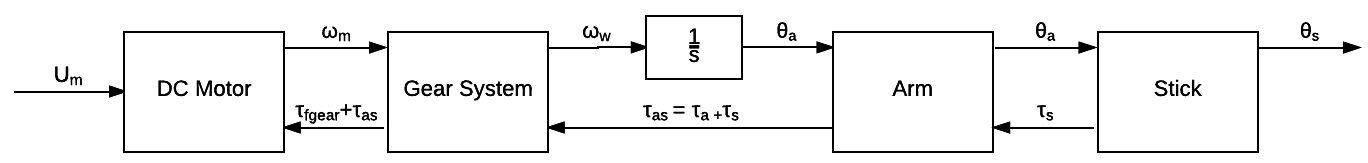
\includegraphics[width=0.95\paperwidth]{figures/modeling/InputOutputSystem.png}
	\caption{Input/output relation of the system.} \label{fig:DCMotorRelation}
\end{figure}

\startexplain
	\explain{$U_m$ is the motor input voltage}{\si{V}}
\stopexplain


\subsubsection{Stick and Arm}
The arm and stick is elements that always appears in the double inverted pendulum setup. The goal is for the arm to apply force on their common joint, which would affect the position of the stick. The physical parameters for the stick and arm is listed cf. table \ref{DimensionsStick}.

\begin{table}[htbp]
\centering
\begin{tabular}{llll}
\hline
Piece           & Parameter & Value & Unit \\ \hline
Stick$_{long}$  & Length    & 0.8   & [m]    \\
Stick$_{long}$  & Weight    & 0.344 & [kg]    \\ 
Stick$_{short}$ & Length    & 0.4   & [m]    \\
Stick$_{short}$ & Weight    & 0.170 & [kg]    \\ 
Arm             & Length    & 0.33  & [m]    \\
Arm             & Weight    & 288   & [kg]   \\ 
\end{tabular}
\caption{Physical parameters of the arm and sticks.}
\label{DimensionsStick}
\end{table}

Some feedback is needed to be able to control the stick trough the arm and gears. Sensors used is implemented as a integrated part of the setup, and will therefore be considered usable and will the choice of the will not be further discussed.

A necessary feedback is the angle between the stick and arm, to know if control is needed to balance the stick. The angle between the stick and arm is detected and sampled via a potentiometer. Equally the position of the arm is needed, this is to determine the amount of change needed to counteract the change in the stick. The position of each potentiometer can be seen cf. figure \ref{fig:InvertedPendulumSetUpPotmeter}. 

\begin{figure} [htbp]
	\centering
	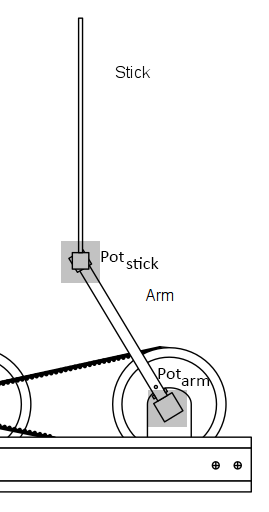
\includegraphics[width=0.35\linewidth]{figures/"Preanalysis&Requirement"/invertedPendulumWithPotmeter.PNG}
	\caption{Diagram of the arm and stick with illustrated sensors.} \label{fig:InvertedPendulumSetUpPotmeter}
\end{figure}



\subsubsection{DC Motor}
To drive the system is a Axem servo motor model F9M2 is attached to the gears. To ensure control precision, the integrated tachometer of the motor is used as feedback. This is done so that it is possible to see the velocity and direction of the motor and relate it to the position of the arm.

	

\subsubsection{Gear System}
Inbetween the DC motor and arm is the gear system. The goal of the gear system is to reduce the ratio between the rotation of the motor versus the arm. The gear system is series of the same size small and big gear connected with belts. The setup is seen cf. figure \ref{fig:InvertedPendulumSetUp}, where the number of gear is illustrated. The parameters of the gear system is listed cf. table \ref{GearSystemParameters}.   

\begin{table}[htbp]
\centering
\begin{tabular}{llll}
\hline
Piece & Parameter & Value & Unit \\ \hline
Gear$_{big}$ & Teeth & 40 & {[}1{]} \\
Gear$_{big}$ & Diameter & 0.12 & {[}m{]} \\
Gear$_{small}$ & Teeth & 12 & {[}1{]} \\
Gear$_{small}$ & Diameter & 0.04 & {[}m{]} \\
Belt & Length & 0.6 & {[}m{]}
\end{tabular}
\caption{Parameters of gear system.}
\label{GearSystemParameters}
\end{table}

The basics of each system in the Inverted Pendulum is now described with its specifications, and the dynamics of the system can therefore be modelled.